\documentclass{ctexbook}
\usepackage{graphicx,floatrow,picinpar,array} 
\usepackage[CJKbookmarks=true,bookmarksnumbered,bookmarksopen,pdftitle={East Indian Company.pdf},pdfauthor=Azur, pdfstartview=FitH,colorlinks=true,linkcolor=black]{hyperref}
\begin{document} 
\tableofcontents  
\part{东印度公司}
\chapter{英属东印度公司}
\section{介绍} 
\begin{figwindow}[1,r,{
    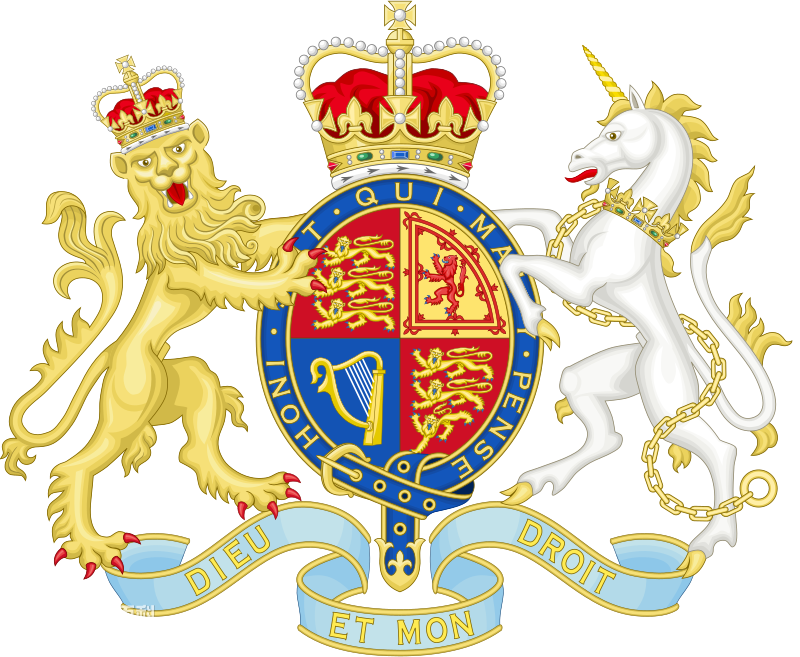
\includegraphics[width=0.3\linewidth]{figure-0.jpg}},{Auspico Regis et Senatus Angliae}]
    \textbf{不列颠东印度公司}(或作“英国东印度公司”,British East India Company,简称BEIC),有时也被称为约翰公司(John Company),1600年12月31日英格兰女王伊丽莎白一世授予该公司皇家特许状,给予它在印度贸易的特权而组成。实际上这个特许状给予东印度贸易的垄断权21年。随时间的变迁东印度公司从一个商业贸易企业变成印度的实际主宰者。在1858年被解除行政权力为止,它还获得了助理政府和军事作用。
\end{figwindow}
\section{影响}
东印度公司的总部在伦敦利德贺街(Leadenhall Street)。它主要建立了英属印度。1717年莫卧尔帝国\footnote{莫卧儿帝国是突厥化的蒙古人帖木儿的后裔巴布尔在印度建立的封建专制王朝。在帝国的全盛时期,领土几乎囊括整个南亚次大陆以及阿富汗等地。莫卧儿帝国上层建筑是穆斯林,而基础则是印度教,波斯语是宫廷、公众事务、外交、文学和上流社会的语言。}皇帝下令免除东印度公司在孟加拉的关税,这给该公司对印度贸易一巨大优势。1757年罗伯特·克莱武爵士在普拉西战役中的决定性胜利使东印度公司成为了一股有力的经济和军事力量。

1760年除少数海岸贸易点外(如本地治里等),法国已被逐出印度。东印度公司对从英国到印度的路途也有兴趣。早在1620年该公司就声称对南非桌山一带有拥有权。后来它占领和统治了圣赫勒拿岛;又参与占领和建设香港和新加坡;以及雇佣威廉·基德对付海盗;另外,公司在印度引入和种植茶。公司历史上其它值得注意的事件包括:将拿破仑关押在圣赫勒拿岛上、伊利胡·耶鲁靠东印度公司发财,而其贸易在英国美洲殖民地则导致了波士顿倾茶事件。
\begin{figure}[!h]
    \begin{floatrow}
        \ffigbox{\caption{1801年至1874年结业前的公司旗帜}}{
\includegraphics[height=0.15\textheight]{figure-1.jpg}}
        \ffigbox{\caption{公司总部设于东印度大楼}}{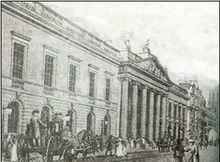
\includegraphics[height=0.15\textheight]{figure-2.jpg}}
    \end{floatrow}
\end{figure}

东印度公司最初的旗帜由圣乔治十字和横杠组成,这有可能是美国国旗的榜样。对历史上两面旗帜的比较说明这个论点有一定的道理。东印度公司的旗帜是1600年代设计的,美国国旗是1777年设计的。东印度公司的船坞为圣彼得堡提供了一个原型,其管理机构的一些成分一直延用到印度的官僚机构,而其公司组织则是早期股份公司的一个成功的典范。该公司对孟加拉地区的财政要求使得当地政府面临1770年的饥荒束手无策,这次饥荒在1770年到1773年间导致上百万人死亡。


\section{历史}
\subsection{创建年代}
东印度公司的全名是“伦敦商人在东印度贸易的公司”。它是由一群有创业心和有影响力的商人所组成。这些商人获得了英国皇家给予他们的对东印度的15年的贸易专利特许。公司共有125个持股人,资金为7.2万英镑。但一开始东印度公司对荷兰的香料贸易威胁很小,因此起初它也未能在东印度建立一个持久的据点。

1608年,公司的船到达苏拉特,并在那里建立了一个贸易点。此后两年中,东印度公司得以在孟加拉湾赛葵的默吉利伯德讷姆建立了它的第一所工厂。由于公司在印度登陆后报告说获得了很高的利润,促使英皇詹姆士一世向其它公司颁发了特许状。

1609年,詹姆士一世向东印度公司发出了一张不设期限的特许状,特许状只会在公司连续三年没有盈利的情况下才会被取消。

\subsection{在印度立足}
英国商人经常在印度洋与荷兰和葡萄牙竞争者发生武装冲突。

1612年东印度公司战胜葡萄牙人,使他们获得莫卧尔帝国皇帝贾汗吉尔的青睐。英国人认识到在远洋作战的胜败是暂时的,因此他们决定在印度本土建立受双方政府支持的立足点。他们要求英皇采取外交措施来达到这个目的。

1615年,英皇詹姆斯一世派托马斯·罗伊爵士拜访贾汗吉尔,贾汗吉尔是印度亚大陆70\%的领域的统治者。这次外交拜访的目的在于在苏拉特和其它地区授予东印度公司独一无二的定居和建立工厂的权利。作为交换,公司愿意向贾汗吉尔提供欧洲市场上的货物和珍品。这次旅程非常成功,贾汗吉尔通过罗伊爵士向詹姆斯一世回信道:

“作为对你的皇室的恩爱我向所有我统治的王国和海港下令接受任何英国商人作为我的朋友。他们可以在任何他们愿意的地方居住,他们享受无限制的自由。不论他们到达哪个海港,葡萄牙或其他人不准打扰他们。不论他们在哪个城市定居,我下令给所有我的总督和长官给予他们任何可以给予的、他们所需要的自由。他们可以任意买卖和向他们的国家运输。
为了加固我们之间的热情和友情,我希望陛下下令您的商人,用他们的船运来各种珍品,和适合我的皇宫的商品,以及您有机会给我传递您的王家信件,以让我欢欣您的健康和事业发展。愿我们的友谊永恒。”
\subsection{扩张}
在这样明显的保护下东印度公司很快就超过了在果阿和孟买建有基地的葡萄牙人。在苏拉特、金奈(1639年)、孟买(1668年)和加尔各答,它建立了大本营。

到1647年为止它在印度已经建立了23个工厂(即基地),有90个雇员。其中大的基地有位于孟加拉的威廉堡、在金奈的圣乔治堡和孟买城堡。
1634年莫卧尔皇帝将他对英国商人的优待扩展到孟加拉地区(1717年甚至完全赦免了孟加拉地区的关税)。东印度公司的主要贸易货物是棉花、丝绸、靛青、硝酸钠和茶。同时东印度公司不断对荷兰人通过马六甲海峡对香料贸易的垄断挑战。

1657年奥利弗·克伦威尔更新了1609年的特许状并对公司的股份分配进行了小的调整。英国皇室复辟后公司的地位更加提高。

1670年查理二世发布了五条法律,授予东印度公司自主占领地盘、铸造钱币、指令要塞和军队、结盟和宣战、签订和平条约和在被占据地区就民事和刑事诉讼进行审判的权利。东印度公司的敌人包括商业竞争者、敌对国家和国内的敌对势力,因此它需要更多的保护权利。从事军事行动的权利因此对公司来说是非常重要的。

1711年,东印度公司在中国广东建立了一个贸易点来使用银换取茶叶。

1680年代公司很快就建立了一支自己的武装力量,其主要人员来于对当地居民的征募。

到1689年为止东印度公司可以说拥有了一个“国家”的特性,它自主地控制着孟加拉、金奈和孟买的统治,拥有可怕的和有威胁性的军事力量。
在1698年,公司拥有了自己的格言“从属于赞助者——英格兰国皇和国会”(Auspico Regis et Senatus Angliae)。
\section{垄断基础}
\subsubsection{鸦片贸易}
在18世纪,中国对鸦片的需求十分之高,而在1773年,东印度公司在孟加拉取得了鸦片贸易的独占权。但由于东印度公司的船只被禁止运送鸦片到中国,所以在孟加拉生产的鸦片要先在加尔各答出售,再在那里运到中国。
尽管中国政府一直禁止鸦片入口,又在1799年重申禁烟,但公司仍从孟加拉透过贸易商和仲介走私鸦片到中国广州等地,平均每年更高达900吨。鸦片源源不绝的输入中国,使中英贸易形成了庞大的逆差,尽管中国输出茶叶和丝绸,仍未能阻止白银大量流出的问题。在1838年,当时鸦片输入中国的数量高达1400吨,中国不得不对走私者处以死刑,并派出钦差大臣林则徐监督禁烟。禁烟与日后的销烟引发了1840年鸦片战争,最终使中国割让香港予英国。
\subsubsection{殖民垄断}
七年战争的结果是法军战败,这挫折了法国的帝国愿望,也削弱了法国境内工业革命的影响。总督罗伯特·克莱芙在印度获得了一次出奇的胜利,战败了那里的法军,重占圣乔治堡。在1763年的巴黎条约中法国在印度的势力仅限于本地治里、马希、雅南等几个没有武装的贸易点。虽然这些小贸易点在此后两百年中保留在法国手中,但法国对印度土地的愿望被打破了,对东印度公司来说这消灭了它的一个大的经济对手。相反的,东印度公司此时拥有一支有纪律、有经验的军队,它得以从其在金奈的基地出发不受任何其它殖民强国的影响保障其从孟加拉到加尔各答的利益。
\subsubsection{地方反抗}
但是当地统治者依然反抗东印度公司的统治。1757年克莱芙在普拉西战役中击败了法国支持的最后一支反抗力量。这次胜利却使得英国与莫卧尔帝国之间的关系变坏了。在奥郎泽布皇帝被废黜后,莫卧尔帝国已经处于分裂过程中。在与公司作战败绩后,莫卧尔皇帝放弃了对孟加拉、比哈尔邦和奥里萨邦的统治。克莱芙由此成为第一位英国在孟加拉的总督。传奇的迈索尔国王提普苏丹也为英军提供了一些烦恼。他是法国的同盟者,在四次英国-迈索尔战争中,他继续反抗东印度公司的统治。1799年英军占领迈索尔,提普苏丹被杀。此后公司继续逐渐削弱当地的反抗势力,占据了孟买及其附近地区。在这些战争中,阿瑟·韦尔斯利,后来的第一代威灵顿公爵,初露锋芒,这是他通向半岛战争和滑铁卢战役的道路的起点。这样英国占据了整个南印度、东印度和西印度。最后的阻力来自北部德里、奥德、拉杰普塔纳和旁遮普的地方势力。公司通过施加压力、挑拨离间、提供可疑的保护等手段有效地防止了这些公国联合抗英。从1757年到1857年印度民族起义东印度公司不断加固其统治,它变得越来越象一个国家,而不象一个贸易企业了。

\chapter{荷属东印度公司}
1602年荷兰建立的具有国家职能、向东方进行殖民掠夺和垄断东方贸易的商业公司。
荷兰东印度公司(Dutch East India Company)成立于1602年3月20日,1799年解散。荷文原文为Vereenig de Oostindische Compagnie,简称VOC,中文全文应译为联合东印度公司。其公司的标帜以V串连O和C,上方的A为阿姆斯特丹的缩写。

1602年荷兰建立的具有国家职能、向东方进行殖民掠夺和垄断东方贸易的商业公司。荷兰东印度公司是第一个可以自组佣兵、发行货币,也是第一个股份有限公司,并被获准与其他国家定立正式条约,并对该地实行殖民与统治的权力。

\begin{figwindow}[2,r,{
    
\includegraphics[width=0.3\linewidth]{figure-3.jpg}},{荷兰东印度公司旗}]
    在荷兰东印度公司成立将近两百年间,总共向海外派出1772艘船,约有100万人次的欧洲人搭乘4789航次的船班前往亚洲地区。平均每个海外据点有二万五千名员工,一万两千名船员。见西欧16~18世纪的海外殖民掠夺。尼德兰联省共和国(States-General of the Netherlands)给予公司在亚洲进行殖民活动21年期限的垄断权,这是世界上第一家跨国公司也是第一个发行股票的公司,这也是世界上第一个特大公司,政府持有股份,有为战争支持薪水,与外国签订条约,铸造货币,建立殖民地等权利,在近200年的时间里,在世界贸易中有重要影响力,每年给政府分红18\%,直到1800年公司正式解散,其财产和债务由巴达维亚共和国(Batavian Republic)承担,公司的殖民地成为荷属东印度,在19世纪又扩展到了整个印度尼西亚群岛,形成了现代意义上的印度尼西亚。
\end{figwindow}

\section{历史背景}
荷兰东印度公司是建立于17世纪欧洲的大航海时代,当时的欧洲各国兴起海上冒险,探寻世界地理,更发展外海的商机。16世纪的葡萄牙在东南亚地区已有殖民地与商业发展,1560年代,一群荷兰商人派浩特曼(Cornelis de Houtman,—1599)至葡萄牙刺探商情,浩特曼回国后这群商人便成立一家公司,利用这个资讯往东印度地区发展,从1595年4月至1602年间,荷兰陆续成立了14家以东印度贸易为重点的公司,为了避免过度的商业竞争,这14家公司于是合并,成为一家联合公司,也就是荷兰东印度公司。荷兰当时的国家议会授权荷兰东印度公司在东起好望角,西至南美洲南端麦哲伦海峡具有贸易垄断权。
\begin{figure}[h]
    \centering
    \caption{荷属东印度公司交易网络}
    \scalebox{1}[0.6]{
    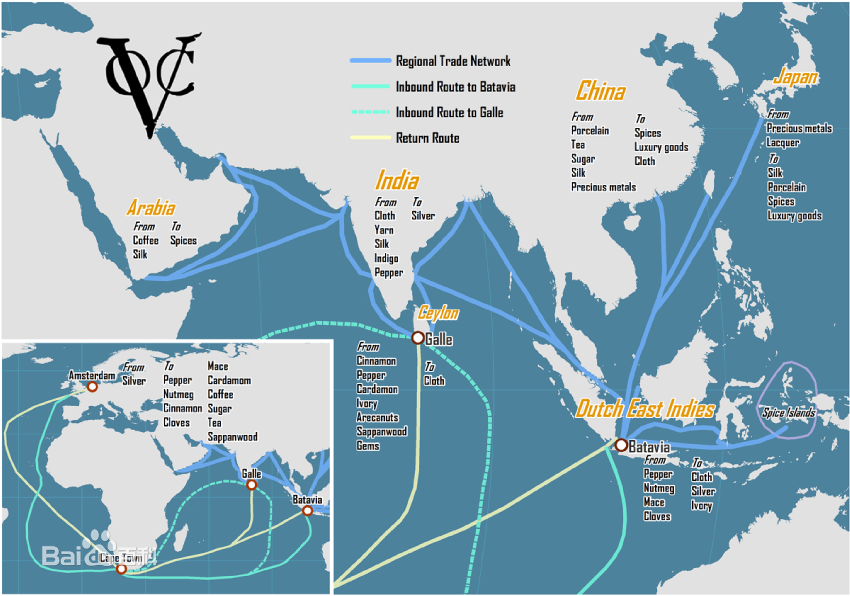
\includegraphics[width=1\linewidth]{figure-4.jpg}}
\end{figure}

荷兰东印度公司由位于阿姆斯特丹、泽兰省的密德堡市、恩克华生市(Enkhuizen)、德夫特市(Delft)、荷恩市(Hoorn)、鹿特丹市(Rotterdam)六处的办公室所组成,其董事会由七十多人组成,但真正握有实权的只有十七人,被称为十七人董事会(Heren XVII),分别是阿姆斯特丹八人、泽兰省4人,其他地区各一人。

荷兰东印度公司是第一个可以自组佣兵、发行货币,也是第一个股份有限公司,并被获准与其他国家定立正式条约,并对该地实行殖民与统治的权力。
荷兰东印度公司在爪哇的巴达维亚(今印尼的雅加达)建立了总部,其他的据点设立在东印度群岛、香料群岛上。

到了1669年时,荷兰东印度公司已是世界上最富有的私人公司,拥有超过150艘商船、40艘战舰、五万名员工、与一万名佣兵的军队,股息高达40\%。认购股份的热潮时,荷兰东印度公司共释出650万荷兰盾供人认购,当时的10盾约等于1英镑,而1660年代荷兰一位教师的年薪约280盾,光阿姆斯特丹一地就认购了一半的股份。
  
\section{与台湾的贸易关系} 

\begin{tabular}{|c@{:}l|c@{:}l|}
    \multicolumn{4}{c}{荷属东印度公司信息表}\\
    \hline
     公司名称 & 荷兰东印度公司 &外文名称 &Dutch East India Company  \\
    \hline
     总部地点 &荷兰阿姆斯特丹 &成立时间 &1602年3月20日  \\
    \hline
     经营范围 &贸易公司 &公司类型 &殖民性掠夺以及垄断性贸易 \\
    \hline 
     员工数 &25000名& 解散时间 &1799年 \\
    \hline
\end{tabular}
\vspace{3mm}

荷兰东印度公司原先在澎湖附近活动,但当时中国明朝政府认为澎湖为其领土,使得荷兰人于1624年转而到当时未有实质政府统治的福尔摩沙(今台湾)大员(今台南市)设立据点,占领台湾的期间由1624年至1662年。当年的建筑如热兰遮城、普罗民遮城等仍留至当代,唯多已倾圯。


\begin{figwindow}[1,r,{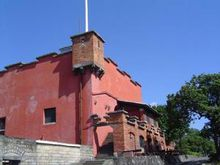
\includegraphics[width=0.3\linewidth]{figure-5.jpg}},{台湾安东尼堡(Fort Anthonio)}]
    占领台湾的目的是为对中国、日本、韩国与东南亚据点的枢钮,并垄断马尼拉(西班牙殖民地)与中国间的贸易。主要的输出贸易内容包括砂糖、鹿皮、鹿肉、鹿角、藤、米,转运贸易内容包括荷兰的金属、药材,巴达维亚的香料、胡椒、琥珀、麻布、棉花、鸦片、锡、铅,中国的丝织品、陶器、黄金。以鹿皮为例,在1634年到1638年短短四年之间,由台湾输出到日本的张数由十一万张成长到十五万张。到了1658年,台湾砂糖的输出量已经足够供应日本与波斯的需要,并增加巴达维亚为输出对象。
\end{figwindow}

荷兰东印度公司亚洲约有35个据点,日本据点的获利为38.8\%排名第一,第二名即是获利25.6\%的台湾,但荷兰东印度公司在这些地方的获利主要是配送给荷兰的股东,而非用回馈当地人或用于当地的建设。

当时在台湾经营贸易的国家除了荷兰,尚有日本人,鉴于日本人的经济竞争,荷兰遂对日本商人课征10\%的税,引起双方不满,甚至发生滨田弥兵卫事件,1628年两方终止贸易,1632年才又恢复,但日本在不久之后进入锁国时代。除此之外,因为荷日两方政府对于其所有领地都有司法权执行的权力,为此两方也发生过冲突。

\end{document} 